\subsection{Web application}\label{sec:web app}
The web application is structured as a normal client-server architecture. After the models have been imported and the server is run, the models are deserialized and stored in the server's main memory.
A client can then connect to the server, at which point the web page itself is server to the client.
The web page contains a simple user interface shown in figure \ref{fig:web page}.

\begin{figure}[h]
	\centering
	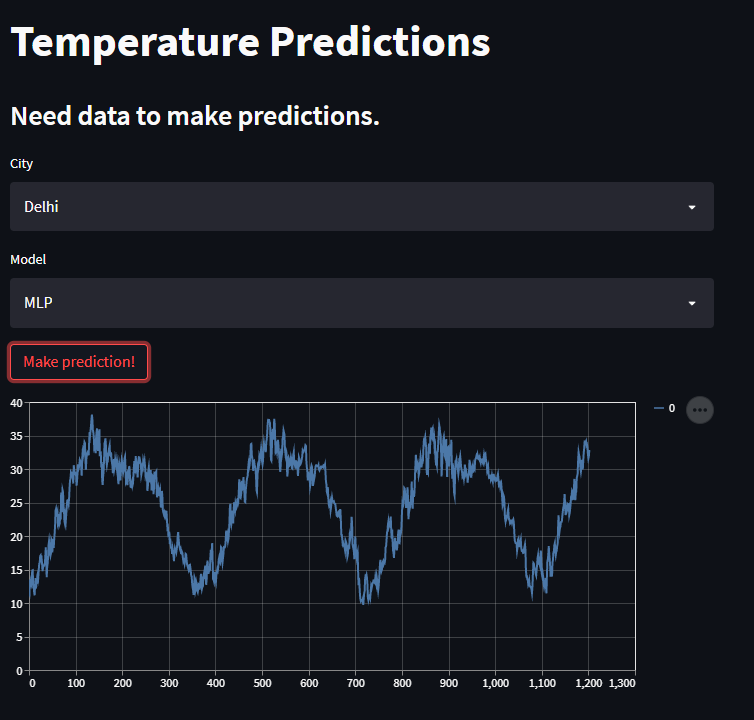
\includegraphics[width=0.5\textwidth]{Web page}
	\caption{The front-end web page.}
	\label{fig:web page}
\end{figure}

The user interface contains two dropdowns: one for selecting the city from which the data was gathered, and one for selecting which machine learning model to use for making a prediction.
Once the user has selected a city and a model, they can click the "Make prediction" button to request a prediction using the selected model.
When the button is clicked, the client sends a request to the server, which, in turn, uses the selected model from the deserialized \texttt{pickle} file to make the prediction. 
Once the prediction has been computed, the response is sent back to the client, and the result is rendered on the web page in the form of a graph.

In order to build this website, we used the open-source Python framework \textit{Streamlit}\cite{streamlit}, which is a framework used to visualize data easily on a web page.
Streamlit also supports scikit-learn\cite{scikit-learn}, PyTorch\cite{pytorch} and TensorFlow\cite{tensorflow}--machine learning frameworks we have used extensively for formatting data and creating and training the models.
This framework allowed us to easily develop and deploy the application interface as well as the back-end functionality using the serialized data and Python objects from the \texttt{pickle}, files described in section \ref{sec:training}.
Instead of having to create the whole website ourselves using HTML, JavaScript and CSS, we can simply write the whole application in Python code, which Streamlit then compiles into a website.
In addition, Streamlit also provides an easy way to host a back-end server, both locally and on the web.

% streamlit